% Mirror: https://github.com/SIGma-UIUC/presentation-format
% --------------------------------------------------------------------
% This is a simple Beamer document that uses beamerthemesigma.sty
% Reading the comments should help you create a presentation even if
% you've never used Beamer before.
% --------------------------------------------------------------------

% Set our document class to Beamer
% \documentclass[aspectratio=169]{beamer}
\documentclass[aspectratio=169, handout]{beamer}
% Add handout option to ignore pauses

% From Jeff E
\usepackage{algo}
% Some more macros
\usepackage{sigmastyle}

\usepackage{tikz}
\usetikzlibrary{graphs}
\usetikzlibrary{arrows.meta}


% Set a title
\title{Quantum Algorithms for Graph Traversals}

% Set a subtitle if you desire
\subtitle{Eulerian Circuits}

% Whoever worked on the presentation:
\author{Sasha Levinshteyn}

% Date looks ugly, so leave blank
\date{}

% An institute name, if you're so inclined
% \institute{University of Illinois Urbana-Champaign}

% Use the SIGma theme for this Beamer presentation
\usetheme{sigma}
% --------------------------------------------------------------------

% Begin document
\begin{document}

% Beamer calls each slide a "frame", defined within the environment:
% \begin{frame}
%   <frame content here>
% \end{frame}

% This frame is just the title.
\begin{frame}
\titlepage
\end{frame}

% A frame with the table of contents.
% This frame's title is "Outline".
\begin{frame}{Outline}
  \tableofcontents
\end{frame}


\begin{frame}{Housekeeping}
    \centering
\includegraphics[width=0.25\textwidth]{qr-code.png}
    \begin{itemize}
        \item Join the Discord!
    \end{itemize}
\end{frame}


\section{Graph Definitions and Problems}
\frame{\sectionpage}


\begin{frame}{Definition of a Graph}
    \begin{itemize}
        \item A graph $\emph{G} = (V, E)$ consists of
        \begin{itemize}
            \item A set of vertices $V$ with $|V| = n$
            \item Binary relations/edges $E$ between vertices with $|E| = m$
        \end{itemize}
    \end{itemize}
    \pause
    \begin{center}
        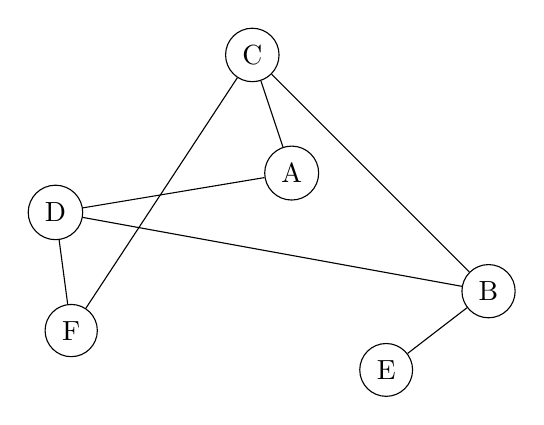
\begin{tikzpicture} [every node/.style={draw,circle}]
            \node (a) at (0.5, 0.5)    {A};
            \node (b) at (3, -1)       {B};
            \node (c) at (0, 2)         {C};
            \node (d) at (-2.5, 0)    {D};
            \node (e) at (1.7, -2)    {E};
            \node (f) at (-2.3, -1.5)   {F};

            \graph[edges={-}] {
                (a) -- (d) -- (b) -- (c);
                (f) -- (c) -- (a);
                (f) -- (d);
                (e) -- (b);
            };
        \end{tikzpicture}
    \end{center}
\end{frame}

\begin{frame}{Degrees and Adjacency}
    \begin{itemize}
        \item If two vertices $u$ and $v$ have an edge between them, they are call \emph{adjacent}. \pause
        \item The \emph{degree} of vertex $v$ is the number of edges with $v$ as an endpoint or the number of vertices adjacent to $v$, denoted $d(v)$. \pause
        \item In a directed graph, the \emph{out-degree} of a vertex $v$ is the number of edges coming out of $v$, denoted $d^+(v)$. \pause
        \item Similarly, the \emph{in-degree} of a vertex $v$ is the number of edges coming into $v$, denoted $d^-(v)$.
    \end{itemize}
\end{frame}

\begin{frame}{Cycles}
    \begin{itemize}
        \item A \emph{cycle} is a sequence of vertices $(v_1, v_2, \dots, v_k, v_1)$ such that \pause
        \begin{itemize}
            \item There is an edge $(v_i, v_{i + 1})$ for $1 \leq i \leq k - 1$ \pause
            \item There is an edge $(v_k, v_1)$ \pause
        \end{itemize}
        \item A cycle of $k$ vertices is called a $k$-cycle.
    \end{itemize}
    \pause
    \begin{center}
        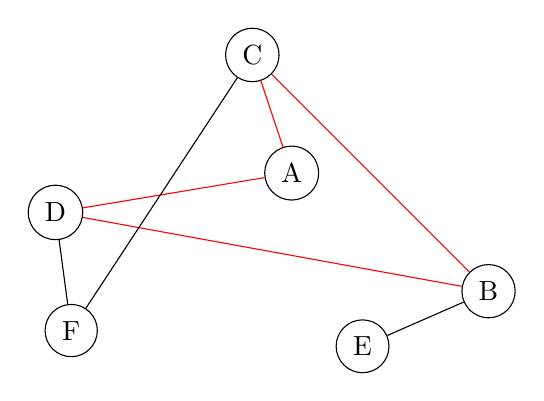
\begin{tikzpicture} [every node/.style={draw,circle}]
            \node (a) at (0.5, 0.5)    {A};
            \node (b) at (3, -1)       {B};
            \node (c) at (0, 2)         {C};
            \node (d) at (-2.5, 0)    {D};
            \node (e) at (1.4, -1.7)    {E};
            \node (f) at (-2.3, -1.5)   {F};

            \graph[edges={-}] {
                (a) --[draw=red] (d) --[draw=red] (b) --[draw=red] (c);
                (f) -- (c) --[draw=red] (a);
                (f) -- (d);
                (e) -- (b);
            };
        \end{tikzpicture}
    \end{center}
\end{frame}

\begin{frame}{Representations of Graphs}
    \begin{itemize}
        \item How do we actually represent a graph mathematically or in an algorithm? \pause
        \item \emph{Adjacency Matrix Model}
        \begin{itemize}
            \item Given $n \times n$ matrix $A \in \{0, 1\}^{n \times n}$ with $A_{ij} = 1$ if there is an edge between vertices $i$ and $j$ and $A_{ij} = 0$ otherwise. 
        \end{itemize} \pause
        \item \emph{Adjacency List Model}
        \begin{itemize}
            \item Given degrees $d(v)$ of each vertex $v$.
            \item Given an array $n(v)$ for each vertex $v$.
        \end{itemize}
    \end{itemize}
\end{frame}

\begin{frame}{Representations of Graphs}
     \begin{itemize}
        \item Let's do this one together!
    \end{itemize}
    \begin{center}
        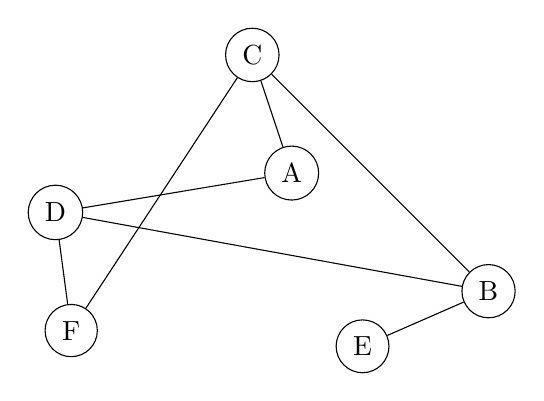
\begin{tikzpicture} [every node/.style={draw,circle}]
            \node (a) at (0.5, 0.5)    {A};
            \node (b) at (3, -1)       {B};
            \node (c) at (0, 2)         {C};
            \node (d) at (-2.5, 0)    {D};
            \node (e) at (1.4, -1.7)    {E};
            \node (f) at (-2.3, -1.5)   {F};

            \graph[edges={-}] {
                (a) -- (d) -- (b) -- (c);
                (f) -- (c) -- (a);
                (f) -- (d);
                (e) -- (b);
            };
        \end{tikzpicture}
    \end{center} 
    \pause
    % \begin{equation*}
    %     \begin{pmatrix}
    %         0 & 0 & 1 & 1 & 0 & 0 \\
    %         0 & 0 & 1 & 1 & 1 & 0 \\
    %         1 & 1 & 0 & 0 & 0 & 1 \\
    %         1 & 1 & 0 & 0 & 0 & 1 \\
    %         0 & 1 & 0 & 0 & 0 & 0 \\
    %         0 & 0 & 1 & 1 & 0 & 0
    %     \end{pmatrix}
    % \end{equation*}
\end{frame}



\begin{frame}{Eulerian Circuits}
    \begin{itemize}
        \item An \emph{Eulerian circuit} or \emph{Eulerian tour} is a closed walk (cycle that can repeat vertices) that uses every edge exactly once. \pause
        \begin{center}
        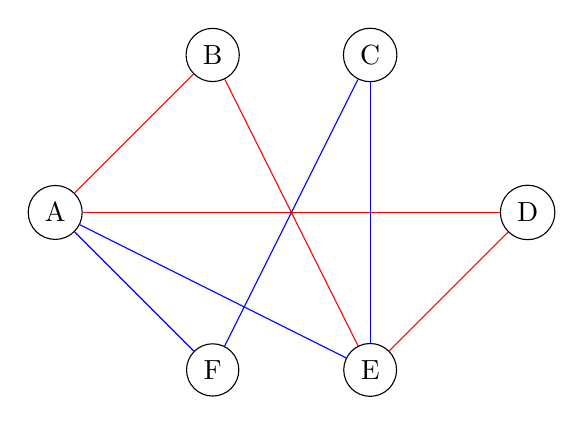
\begin{tikzpicture} [every node/.style={draw,circle}]
            \node (a) at (-3, 0)    {A};
            \node (b) at (-1, 2)       {B};
            \node (c) at (1, 2)         {C};
            \node (d) at (3, 0)    {D};
            \node (e) at (1, -2)    {E};
            \node (f) at (-1, -2)   {F};

            \graph[edges={-}] {
                (a) --[draw=red] (b) --[draw=red] (e) --[draw=red] (d) --[draw=red] (a) --[draw=blue] (e) --[draw=blue] (c) --[draw=blue] (f) --[draw=blue] (a)
            };
        \end{tikzpicture}
    \end{center}
    \end{itemize}
\end{frame}

\begin{frame}{Eulerian Circuit Problem}
    \begin{itemize}
        \item \emph{Eulerian Circuit Problem}: Determine if a graph $G$ has an Eulerian circuit (and is thus Eulerian). \pause
        \item Unlike the Hamiltonian cycle problem from last week, this is very much NOT NP-hard.
        \item As it turns out, even classically, we can do this in $O(n^2)$ time in the adjacency matrix model and $O(n)$ time in the adjacency list model.
    \end{itemize}
\end{frame}

\begin{frame}{Euler's Theorem (The Graph Theory One (The Eulerian Circuits One))}
    \begin{itemize}
        \item A (connected undirected) graph has an Eulerian circuit if and only if every vertex has even degree.
    \end{itemize}
\end{frame}

\begin{frame}{Euler's Theorem Proof}
    \begin{itemize}
        \item Assume that we have a graph $G = (V, E)$ with $|V| = n$ and $|E| = m$.  \pause
        \item Assume $G$ has an Eulerian circuit $v_1 \to v_2 \to \dots \to v_m \to v_1$, where the vertices may repeat but the edges may not. \pause
        \begin{itemize}
            \item The total amount of vertices (repeats included) in the circuit must be equal to the total amount of edges in the graph. \pause
            \item The degree of a vertex is equal to the number of edges connected to it. \pause
            \item We can go through the circuit and increment the degree of a vertex each time we encounter an edge that uses that vertex. \pause
            \item Each time we encounter a vertex, we encounter exactly 2 adjacent edges, which must all be unique since this is an Eulerian circuit. \pause
            \item So, each vertex in $G$ has even degree.
        \end{itemize}
    \end{itemize}
\end{frame}

\begin{frame}{Euler's Theorem Proof}
    \begin{itemize}
        \item Assume that we have a graph $G = (V, E)$ with $|V| = n$ and $|E| = m$. \pause
        \item Assume all vertices of $G$ have even degree. \pause
        \begin{itemize}
            \item Induct on the number of vertices $n$. \pause
            \item Base Case: A graph with 1 vertex and thus 0 edges vacuously has an Eulerian circuit. \pause
            \item Assume that every graph with $k < n$ vertices all with even degree has an Eulerian circuit.
        \end{itemize}
    \end{itemize}
\end{frame}

\begin{frame}{Euler's Theorem Proof}
    \begin{itemize}
        \item Assume all vertices of $G$ have even degree.
        \begin{itemize}
            \item Now, we have $n$ vertices. \pause
            \item Choose some vertex $v_0$ and remove it and its adjacent edges to create a new graph $G'$. \pause
            \item We must have removed an even amount $2x$ of edges to an even amount of other vertices $v_1, v_2, \dots, v_{2x - 1}, v_{2x}$. \pause
            \item Split these other vertices into $x$ pairs $(v_{2i - 1}, v_{2i})$. \pause
            \item For each pair, if they were already connected with an edge, remove that edge, otherwise, add that edge. \pause
            \item Now, each of the affected vertices in $G'$ has either lost one edge and gained one edge or lost two edges, maintaining the even degree property.
        \end{itemize}
    \end{itemize}
\end{frame}

\begin{frame}{Euler's Theorem Proof}
    \begin{itemize}
        \item Assume all vertices of $G$ have even degree.
        \begin{itemize}
            \item $G'$ is now composed of some number of connected components, each containing only vertices of even degree.
            \item By the inductive hypothesis, each of these connected components has an Eulerian circuit. \pause
            \item Consider the pairs of vertices $(v_{2i - 1}, v_{2i})$ we connected. \pause
            \item If we remove the edge and add $v_0$ and its adjacent edges again, we can go from $v_{2i - 1}$ to $v_0$ to $v_{2i}$ instead. \pause
            \item Consider the pairs of vertices $(v_{2j - 1}, v_{2j})$ we disconnected. \pause
            \item If we readd the edge and add $v_0$ and its adjacent edges again, we can go from (the Eulerian circuit of the CC $v_{2j - 1}$ was a part of) to $v_{2j - 1}$ to $v_0$ to $v_{2j}$ to (the Eulerian circuit of the CC $v_{2j}$ was a part of if different) to $v_{2j - 1}$, reconstructing an Eulerian circuit in $G$.
        \end{itemize}
    \end{itemize}
\end{frame}



% \begin{frame}{Hamiltonian Cycles}
%     \begin{itemize}
%         \item
%     \end{itemize}
% \end{frame}



\begin{frame}{}
      \begin{center}
    {\color{sigma@mainblue} \LARGE Questions?}
  \end{center}
\end{frame}

\section{Quantum Computing Speedrun}
\frame{\sectionpage}

\begin{frame}{Motivation}
    \begin{itemize}
        \item I firmly believe we should add the word quantum in front of everything, obviously! \pause
        \item If $P = NP$, classical cryptography breaks but quantum cryptography... \pause
        \begin{itemize}
            \item Come to SIGQuantum tomorrow at 6 pm to find out! \pause
        \end{itemize}
        \item Entanglement and superposition can be exploited to store and manipulate data, exploring multiple paths simultaneously, in ways that classical computers can't \pause
        \item We can (theoretically) get much faster runtimes for algorithms that require certain kinds of computation
    \end{itemize}
\end{frame}

\begin{frame}{Quantum Algorithms}
    \begin{itemize}
        \item A \emph{quantum algorithm} is represented by a \emph{quantum circuit} that... \pause
        \begin{itemize}
            \item Acts on some amount of input \emph{qubits} \pause
            \item Composed of \emph{quantum gates} that transform the qubits \pause
            \item Ends with a \emph{measurement} on some of the qubits \pause
        \end{itemize}
    \end{itemize}
    \begin{center}
    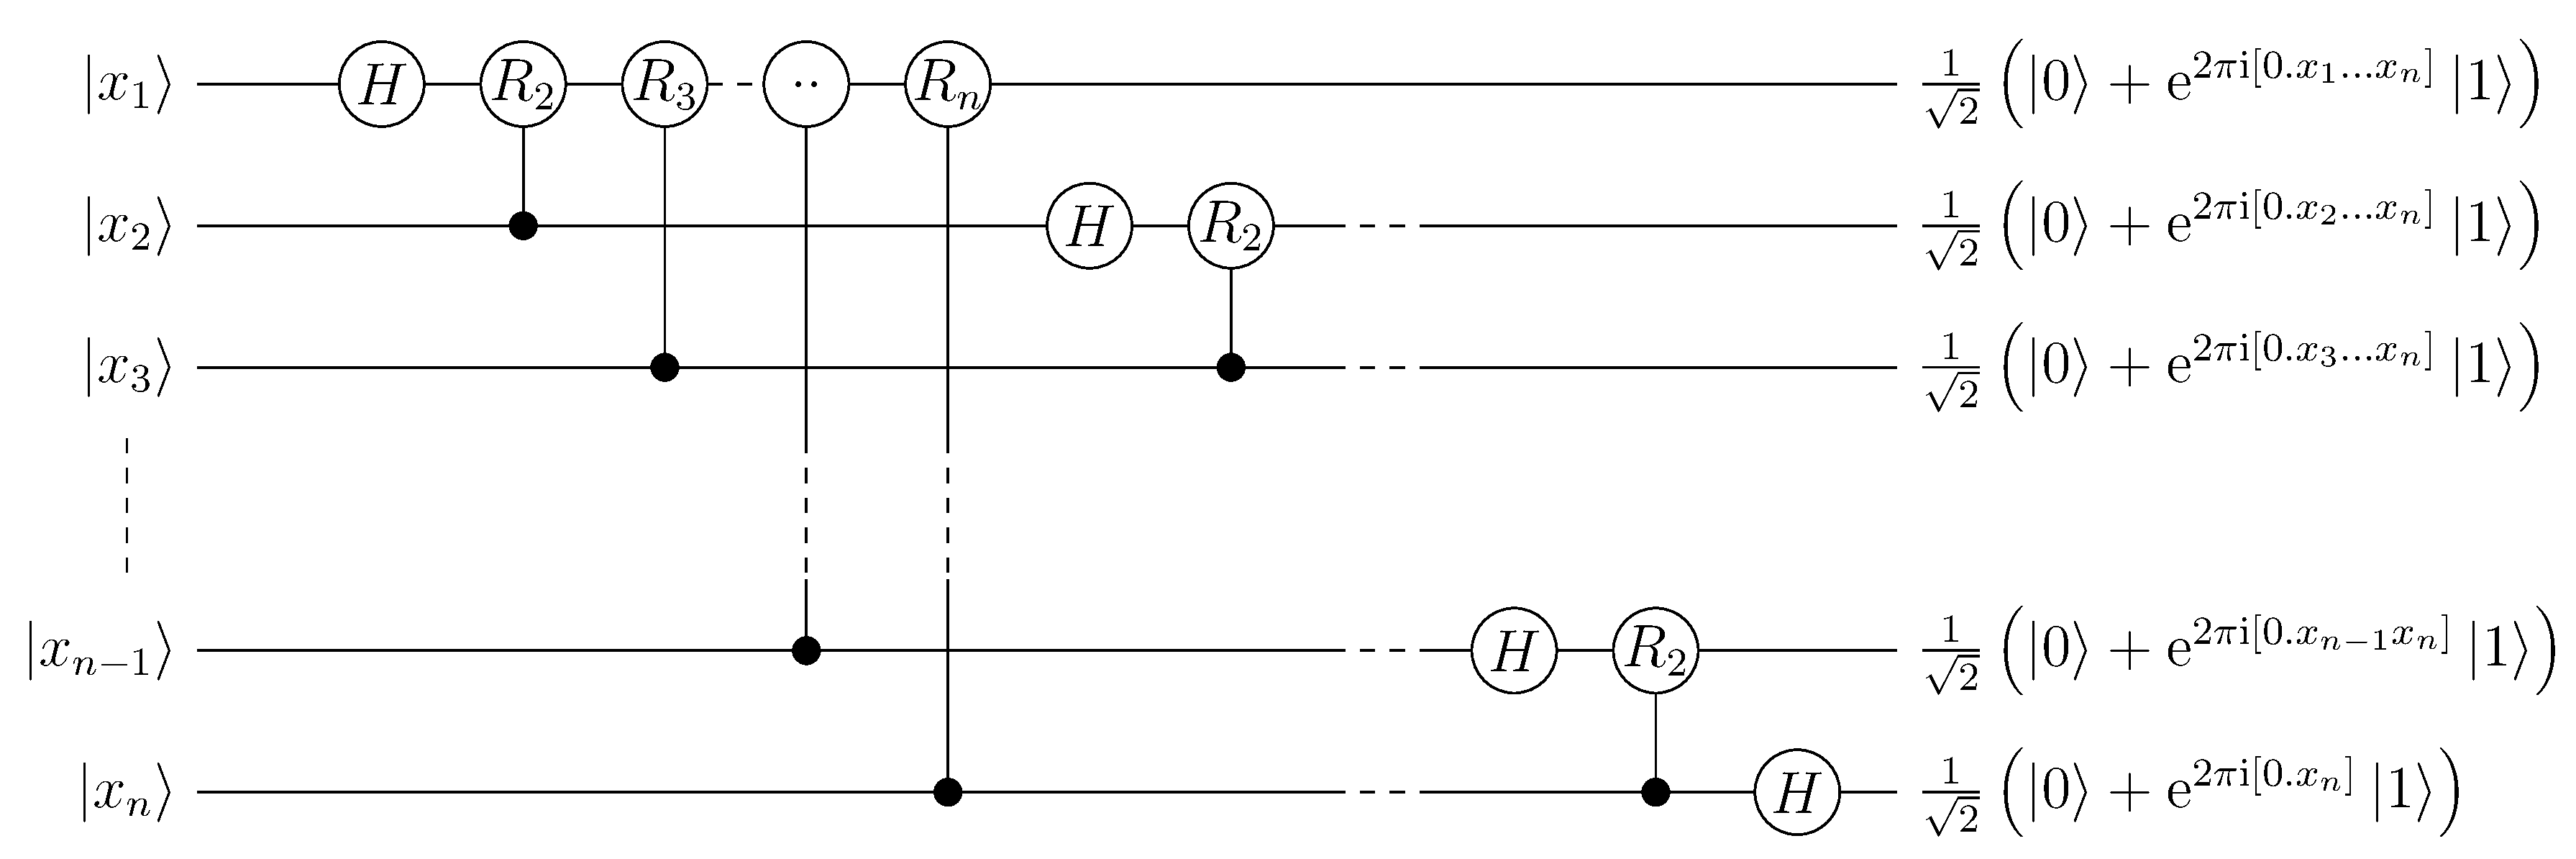
\includegraphics[width=100mm]{QFT.png} \cite{site:qft}
    \end{center}
\end{frame}

\begin{frame}{Qubits, Gates, and Other Scary Words}
    \begin{itemize}
        \item A qubit is a \textbf{vector}! \pause
        \begin{itemize}
            \item When working with a single qubit, the standard basis vectors are
            \begin{equation*}
                \ket{0} = \begin{pmatrix}
                1 \\
                0
                \end{pmatrix}
                \text{ and }
                \ket{1} = \begin{pmatrix}
                0 \\
                1
                \end{pmatrix}
            \end{equation*} \pause
            \item A given unit vector can be represented as a linear combination:
            \begin{equation*}
                \ket{\psi} = \alpha \ket{0} + \beta \ket{1} = \begin{pmatrix}
                \alpha \\
                \beta
                \end{pmatrix},
                |\alpha|^2 + |\beta|^2 = 1, \alpha, \beta \in \mathbb{C}
            \end{equation*}
            \pause
            \item When measured in the standard basis, the qubit will collapse into the $\ket{0}$ state with probability $\alpha^2$ or the $\ket{1}$ state with probability $\beta^2$
        \end{itemize}
    \end{itemize}
\end{frame}

\begin{frame}{Qubits, Gates, and Other Scary Words}
\begin{itemize}
    \item A gate is a \textbf{matrix}! \pause
    \item Most gates that you will encounter are... \pause
    \begin{itemize}
        \item Unitary matrices: $UU^\dag = U^\dag U = I$
        \item Hermitian matrices: $H = H^\dag$
    \end{itemize} \pause
    \item Quantum algorithms are largely just matrices being multiplied to input vectors in ways that compute many values simultaneously. \pause
    \item Don't let the physicists scare you!
\end{itemize}
\end{frame}
        

\begin{frame}{Qubits, Gates, and Other Scary Words}
\begin{center}
    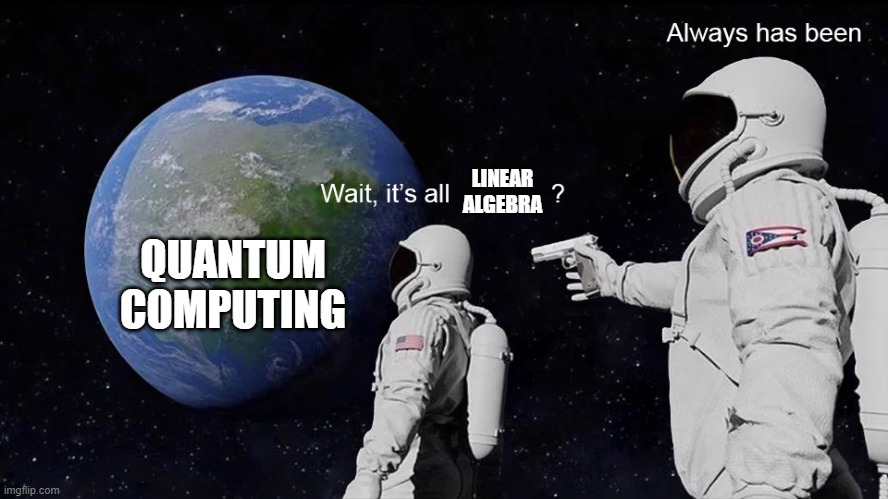
\includegraphics[width=120mm]{QCLA.jpg}
\end{center}
\end{frame}

\begin{frame}{}
      \begin{center}
    {\color{sigma@mainblue} \LARGE Questions?}
  \end{center}
\end{frame}

\section{Quantum Algorithms}
\frame{\sectionpage}

\begin{frame}{Note About Quantum Algorithms}
\begin{itemize}
    \item You don't have to know many details of quantum computing to understand most quantum algorithms. \pause
    \item Most quantum algorithms for graph theory problems do most of the work by calling the same few critical quantum algorithms. \pause
    \item If you know what those smaller quantum algorithms do, you can blackbox them away.
\end{itemize}
\end{frame}

\begin{frame}{Notions of Complexity}
\begin{itemize}
    \item The \emph{quantum query complexity} of a graph algorithm is the number of queries it makes to the adjacency matrix or list representing the graph. \pause
    \item The \emph{quantum time complexity} of a graph algorithm is the number basic quantum operations it makes.
\end{itemize}
\end{frame}

\begin{frame}{Grover's Algorithm}
\begin{itemize}
    \item Quantum Search Problem: Suppose we have a function $f: \{0, 1, \dots, n - 1\} \to \{0, 1\}$ such that $f(x) = 1$ for at most one $x$, which we will call $\omega$. Find this $x$ if it exists. \pause
    \item Grover's algorithm can do this using $O(\sqrt{n})$ evaluations of $f$, beating the classical $O(n)$ evaluations. \pause
    \item $U_\omega\ket{x} = (-1)^{f(x)}\ket{x}$
\end{itemize}
\begin{center}
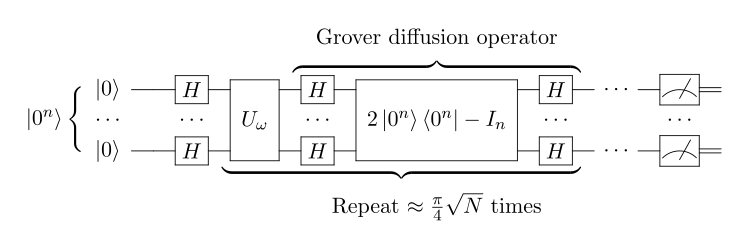
\includegraphics[width=120mm]{Grover.png} \cite{site:grover}
\end{center}
\end{frame}

\begin{frame}{Reducing Error}
\begin{itemize}
    \item Quantum algorithms are not always correct. \pause
    \item They output an incorrect answer with a probability $p$. \pause
    \item To get the probability of an incorrect answer down to $\epsilon$, we need to repeat $r$ times so that $p^r \leq \epsilon$, so we can make the probability of an incorrect answer less than $\frac{1}{n}$ by repeating each quantum subroutine $r = O(\log n)$ times \pause
    \item So, if we have a quantum algorithm with $O(f(n))$ quantum query complexity, it will typically have $O(f(n) \log n)$ quantum time complexity. \pause
    \item Grover's algorithm actually needs an extra logarithmic factor, so it will have $O(\sqrt{n} \log^2 n)$ quantum time complexity. 
\end{itemize}
\end{frame}



\section{Eulerian Circuit Problem Quantum Algorithm}
\frame{\sectionpage}

\begin{frame}{Adjacency List Model}
\begin{itemize}
    \item Algorithm \cite{site:dorn} \pause
    \begin{itemize}
        \item The degree of every vertex is given. \pause
        \item Search the list of degrees for an odd number using a simple quantum search. \pause
        \item If we find an odd number, it is not Eulerian. \pause
        \item Otherwise, it is Eulerian. \pause
    \end{itemize}
    \item Complexity \pause
    \begin{itemize}
        \item The quantum search requires $O(\sqrt{n})$ queries to the list of degrees, making this algorithm have $O(\sqrt{n})$ quantum query complexity. \pause
        \item As this search utilizes Grover's algorithm, the algorithm will have $O(\sqrt{n} \log^2 n)$ quantum time complexity.
    \end{itemize}
\end{itemize}
\end{frame}

\begin{frame}{Adjacency Matrix Model}
\begin{itemize}
    \item Algorithm \pause
    \begin{itemize}
        \item This time, we don't know the degrees right away. \pause
        \item Grover's algorithm in combination with a classical algorithm can be used to compute the parity of each column. \pause
        \item If we find an odd number, it is not Eulerian. \pause
        \item Otherwise, it is Eulerian. \pause
    \end{itemize}
    \item Complexity \pause
    \begin{itemize}
        \item This algorithm will have $O(n^{1.5})$ quantum query complexity. \pause
        \item As this search utilizes Grover's algorithm, the algorithm will have $O(n^{1.5} \log^2 n)$ quantum time complexity.
    \end{itemize}
\end{itemize}
\end{frame}


% \begin{frame}{Weekly Brainteaser}
%     After the revolution, each of the 66 citizens of a certain city, including the king, has a salary of 1. King cannot vote, but has the power to suggest changes to the distribution of salaries. Each person's salary must be a \textbf{non-negative whole number of dollars}, and the salaries must sum to 66. He suggests a new salary plan for every person including himself in front of the city. Citizens are greedy, and vote yes if their salary is raised, no if decreased, and don't vote otherwise. The majority vote wins. The king proposes a series of plans to maximize his salary. \textbf{What is the king's maximum salary?}
% \end{frame}

\begin{frame}{Brainteaser}
    13 Apples, 15 Bananas and 17 Cherries are put in a hat. Inside the hat, if two fruits of different type collide, they both get converted into the third type. For example 1 apple and 1 banana can collide to form 2 cherries. Can a sequence of collisions lead to all 45 fruits having just one type?
\end{frame}



\begin{frame}[allowframebreaks]{Bibliography}
    \tiny
    \bibliography{refs}
    \bibliographystyle{alpha}
\end{frame}


\end{document}